\documentclass{report}

\usepackage{graphicx}
\usepackage{amssymb}
\usepackage{amsmath}
\usepackage{mleftright}
\usepackage{mathtools}
\usepackage[hidelinks]{hyperref}
\usepackage[margin=1in]{geometry}
\usepackage{changepage}
\usepackage{listings}
\usepackage{xcolor}
\usepackage{roboto}

\graphicspath{ {./images/} }

\title{Computer Science 275 Project \\ Topic 3 : University Course Registration System}

\author{Carter Clifton, John Kendall, Chaofan Wang, Miller Zhang}
\date{Winter 2025}

\definecolor{dkgreen}{rgb}{0,0.6,0}
\definecolor{gray}{rgb}{0.5,0.5,0.5}
\definecolor{mauve}{rgb}{0.58,0,0.82}
\lstset{language=SQL,
    basicstyle={\small\ttfamily},
    belowskip=3mm,
    breakatwhitespace=true,
    breaklines=true,
    classoffset=0,
    columns=flexible,
    commentstyle=\color{dkgreen},
    framexleftmargin=0.25em,
    keywordstyle=\color{blue},
    numbers=left,
    numberstyle=\tiny\color{gray},
    showstringspaces=false,
    stringstyle=\color{mauve},
    tabsize=3,
    xleftmargin=1em,
    frame=single
}

\makeatletter
\newenvironment{fullcenter}%
    {\@parboxrestore%
    \begin{adjustwidth}{}{\leftmargin}%
    \begin{center}%
    }{\end{center}%
    \end{adjustwidth}%
    }
\makeatother

\newcommand{\usection}[1]{\section*{#1}
\addcontentsline{toc}{section}{\protect\numberline{}#1}}

\newcommand{\usubsection}[1]{\subsection*{#1}
\addcontentsline{toc}{subsection}{\protect\numberline{}#1}}

\newcommand{\uchapter}[1]{\chapter*{#1}
\addcontentsline{toc}{chapter}{\protect\numberline{}#1}}

\begin{document}

\maketitle{}

\tableofcontents

\uchapter{Enchanced Entity-Relationship (EER) Diagram}

\usection{EER Diagram}

\begin{center}
    \resizebox{\columnwidth}{!}{%
    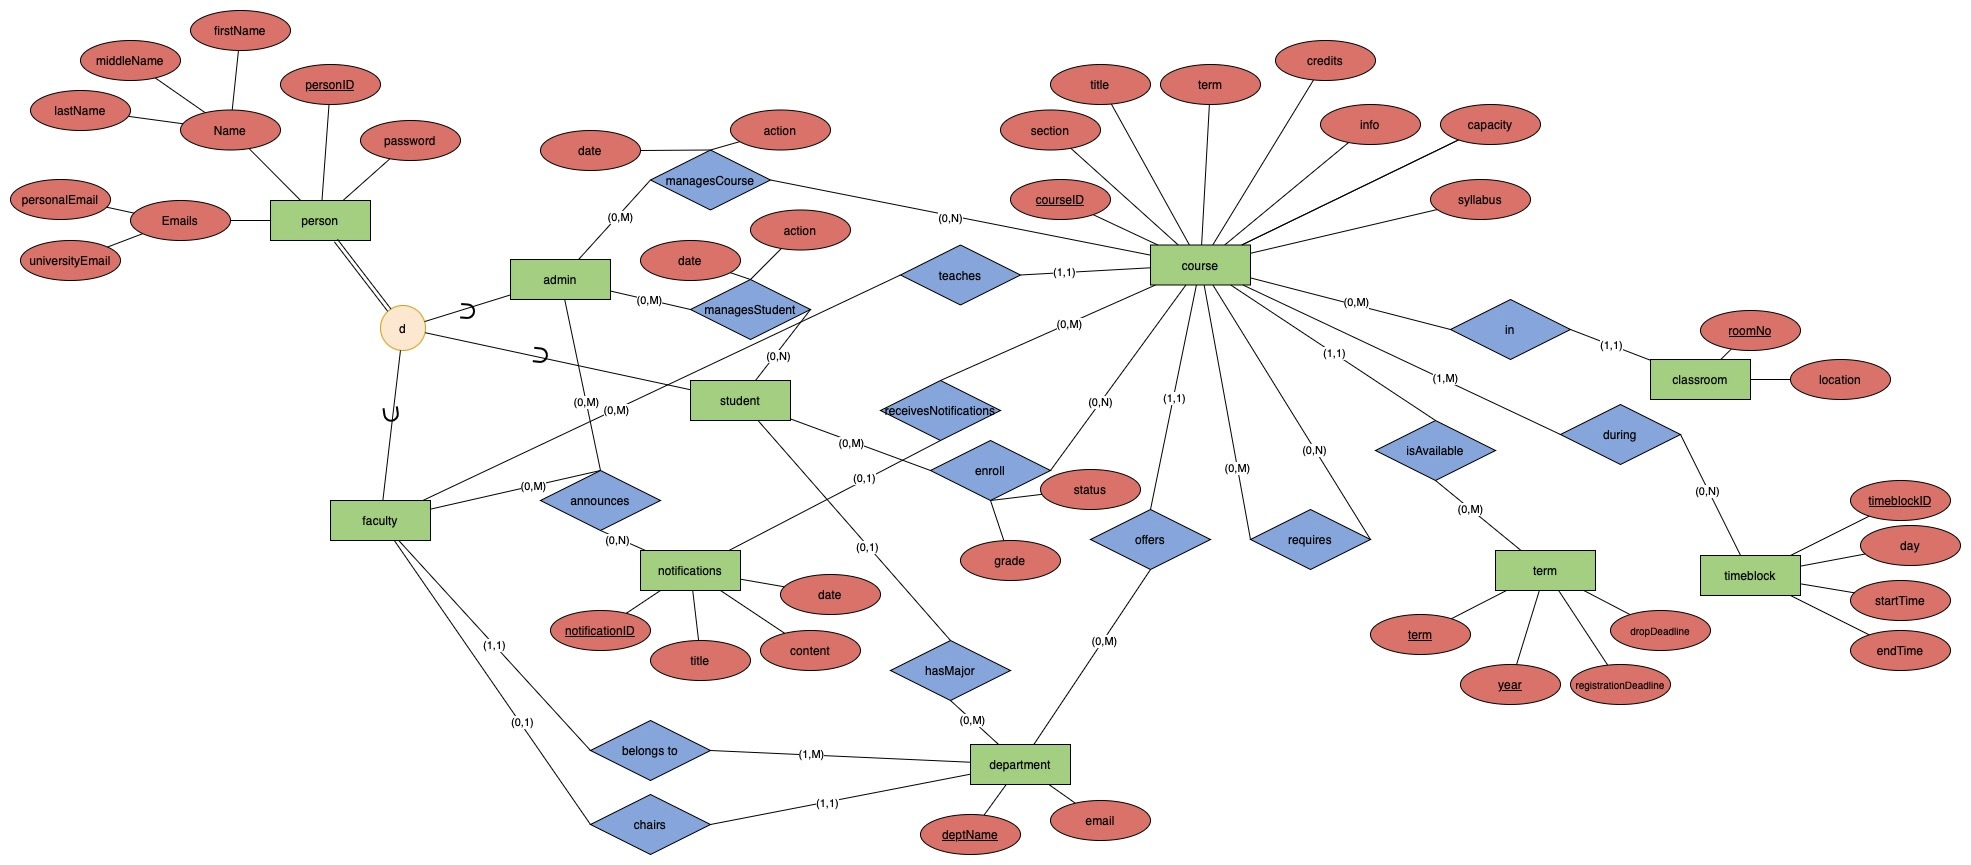
\includegraphics{eer_diagram.jpg}%
    }
\end{center}

\usection{Assumptions}

\begin{itemize}
    \item A person must be either a faculty member, a student, or an admin. They cannot be more than one, or none of these.
    \item A faculty member does not have to each any courses.
    \item A student does not need to take any courses.
    \item A student, faculty, and admin cannot have the same ID. This value is unique across all tables.
\end{itemize}

\usection{Entities and Attributes}

\begin{itemize}
    \item \textbf{Person}
    \begin{itemize}
        \item Attributes: \underline{personID}, Name (firstName, middleName, lastName), Emails (personalEmail, universityEmail), password
        \item Specializations:
        \begin{itemize}
            \item \textbf{Admin}
            \item \textbf{Student}
            \item \textbf{Faculty}
        \end{itemize}
    \end{itemize}
    \item \textbf{Course}
    \begin{itemize}
        \item Attributes: \underline{courseID}, section, title, term, credits, info, capacity, syllabus
    \end{itemize}
    \item \textbf{Department}
    \begin{itemize}
        \item Attributes: \underline{deptName}, email
    \end{itemize}
    \item \textbf{Classroom}
    \begin{itemize}
        \item Attributes: \underline{roomNo}, location
    \end{itemize}
    \item \textbf{Term}
    \begin{itemize}
        \item Attributes: \underline{term}, \underline{year}, registrationDeadline, dropDeadline
    \end{itemize}
    \item \textbf{Timeblock}
    \begin{itemize}
        \item Attributes: \underline{timeblockID}, day, startTime, endTime
    \end{itemize}
    \item \textbf{Notifications}
    \begin{itemize}
        \item Attributes: \underline{notificationID}, title, content, date
    \end{itemize}
\end{itemize}

\usection{Relationships}

\begin{itemize} 
    \item Faculty --- (0,1) --- \textbf{Chairs} --- (1,1) --- Department
    \item Faculty --- (1,1) --- \textbf{BelongsTo} --- (1,M) --- Department
    \item Faculty --- (0,M) --- \textbf{Teaches} --- (1,1) --- Course
    \item Student --- (0,M) --- \textbf{Enroll} --- (0,N) --- Course
    \begin{itemize}
        \item Attributes: grade, status
    \end{itemize}
    \item Student --- (0,1) --- \textbf{hasMajor} --- (0,M) --- Department
    \item Department --- (0,M) --- \textbf{Offers} --- (1,1) --- Course
    \item Course --- (0,M) --- \textbf{Requires} --- (0,N) --- Course
    \item Course --- (0,M) --- \textbf{In} --- (1,1) --- Classroom
    \item Course --- (1,M) --- \textbf{During} --- (0,N) --- Timeblock
    \item Course --- (1,1) --- \textbf{IsAvailable} --- (0,M) --- Term
    \item Admin --- (0,M) --- \textbf{ManagesCourse} --- (0,N) --- Course
    \begin{itemize}
        \item Attributes: date, action
    \end{itemize}
    \item Admin --- (0,M) --- \textbf{ManagesStudent} --- (0,N) --- Student
    \begin{itemize}
        \item Attributes: date, action
    \end{itemize}
    \item Faculty, Admin --- (0,M) --- \textbf{Announces} --- (0,1) --- Notifications
    \item Course --- (0,M) --- \textbf{ReceivesNotification} --- (0,1) --- Notifications
\end{itemize}



\uchapter{Relational Model}

\usection{Relational Model}

\begin{center}
    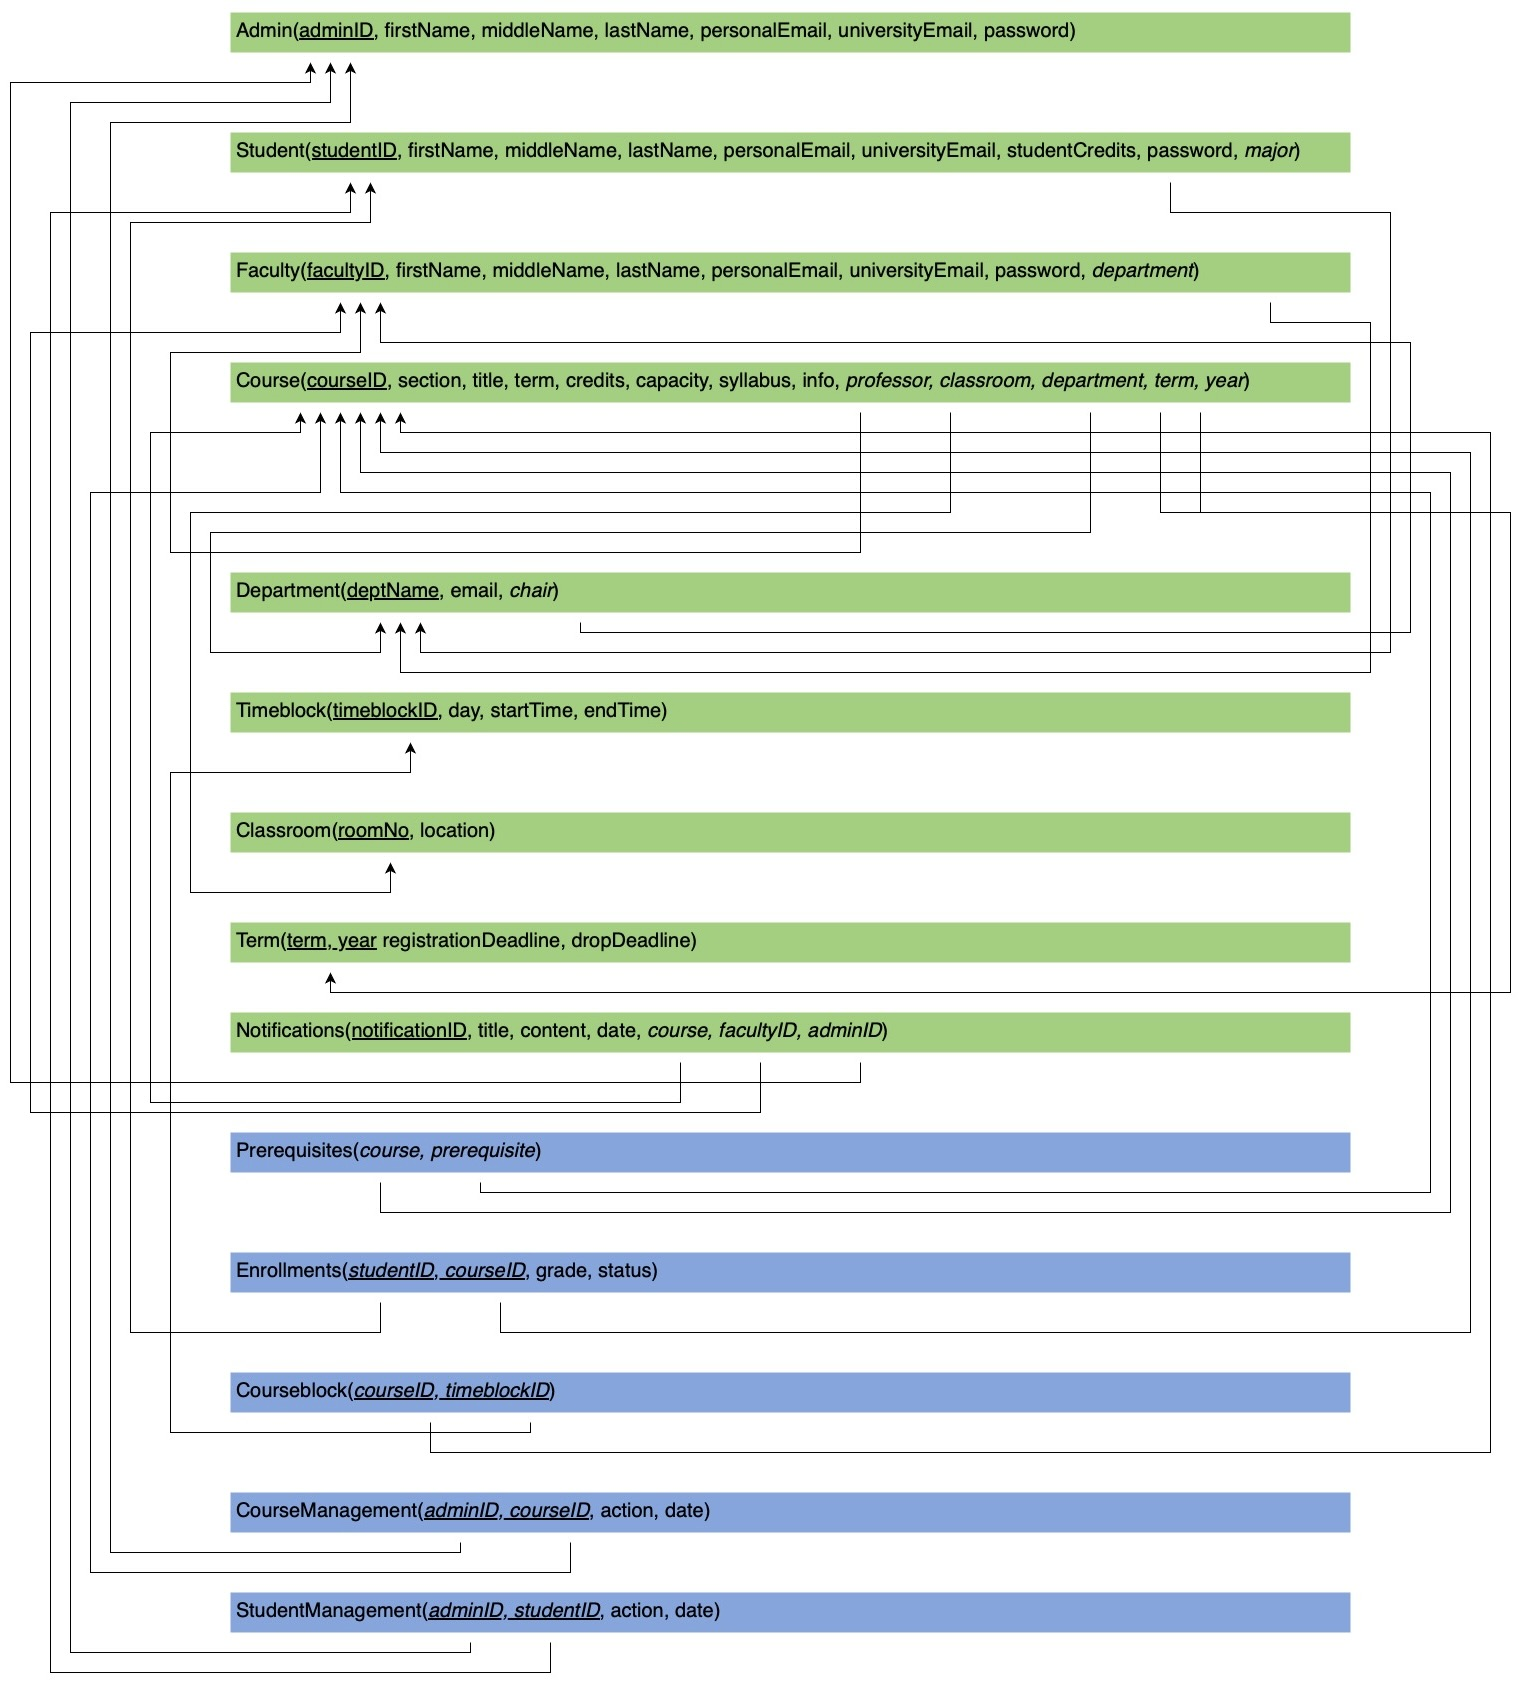
\includegraphics[width=\textwidth, height=0.68\textheight, keepaspectratio]{relational_model.jpg}
\end{center}

\usection{Mapping the EER Diagram to the Relational Model}

\begin{itemize}

    \item Generalization:
    \begin{itemize}
        \item The \textbf{Person} entity is generalized into three entities: \textbf{Student}, \textbf{Faculty}, and \textbf{Admin}. While this means that we do have some duplicate attributes in these entities, we will not need to any joins in order to retrieve all the information about these entities. This is helpful since these entities are referenced frequently.
    \end{itemize}

    \item Composite Attributes:
    \begin{itemize}
        \item The \textbf{Person} entity (and thus the \textbf{Student}, \textbf{Faculty}, and \textbf{Admin} entities) have two sets of composite attributes, being \textbf{Name}, and \textbf{Emails}. We opted to separate these into multiple attributes, this means that \textbf{Name} became the attributes \textbf{(firstName, middleName, lastName)}, and \textbf{Emails} became the attributes \textbf{(personalEmail, universityEmail)}.
    \end{itemize}

    \item Weak Entities:
    \begin{itemize}
        \item We do not have any weak entities in our EER diagram to map.
    \end{itemize}

    \item Recursive Relationships:
    \begin{itemize}
        \item The \textbf{Requires} relationship is a recursive relationship since it contains any prerequisites a course may have. This is also a many-to-many relationship since a course can have multiple prerequisites, and a course can be a prerequisite for many other courses. Since this relationship is many-to-many, we must create a new table called \textbf{Prerequisites}. This table contains only the \textbf{course}, and \textbf{prerequisite}.
    \end{itemize}

    \item 1 - 1 Binary Relationships:
    \begin{itemize}
        \item The \textbf{Chairs} relationship is a 1 - 1 binary relationship since a department can only have one chair, and a professor can only be the chair of one department. This relationship is represented by putting the \textbf{Faculty} table's primary key (\textbf{facultyID}) into the the table for \textbf{Department} as a foreign key.
    \end{itemize}

    \item 1 - M Binary Relationships:
    \begin{itemize}
        \item The \textbf{Teaches} relationship is a 1 - M binary relationship since a professor can teach multiple courses, but a course can only have one professor teaching it. This relationship is represented by putting the primary key of \textbf{Faculty} (\textbf{facultyID}) into the \textbf{Course} table as a foreign key.
        \item The \textbf{In} relationship is a 1 - M binary relationship since a course can only take place in one room, but a room can have multiple courses take place in it. This relationship is represented by putting the primary key of \textbf{Classroom} (\textbf{roomNo}) into the \textbf{Course} table as a foreign key.
        \item The \textbf{Offers} relationship is a 1 - M binary relationship since a department offers many different courses, but each course belongs to only one department. This relationship is represented by putting the primary key of \textbf{Department} (\textbf{deptName}) into the \textbf{Course} table as a foreign key.
        \item The \textbf{hasMajor} relationship is a 1 - M binary relationship since a student can only declare one major, but a department has many students taking their program. This relationship is represented by putting the primary key of \textbf{Department} (\textbf{deptName}) into the \textbf{Student} table as a foreign key.
        \item The \textbf{belongsTo} relationship is a 1 - M binary relationship since a faculty member belongs to only one department, but a department has many faculty members employed. This relationship is represented by putting the primary key of \textbf{Department} (\textbf{deptName}) into the \textbf{Faculty} table as a foreign key.
        \item The \textbf{receivesNotification} relationship is a 1 - M binary relationship since a course can have multiple notifications, but a notification is only for at most one class. This relationship is represented by putting the primary key of \textbf{Course} (\textbf{courseID}) into the \textbf{Notifications} table as a foreign key.
        \item The \textbf{isAvailable} relationship is a 1 - M binary relationship since a course can only be available in one term (if a course like CSCI 275 is offered in multiple terms / years, it needs to be in the course table multiple times), but a term can have many courses available in it. This relationship is represented by putting the primary keys of \textbf{Term} (\textbf{term}, \textbf{year}) into the \textbf{Course} table as a foreign key.
        \item The \textbf{Announces} relationship is a 1 - M binary relationship since a a notification can only have one sender (Admin or Faculty), but a sender (Admin or Faculty) can send multiple notifications. This relationship is represented by putting the primary keys of \textbf{Faculty} and \textbf{Admin} (\textbf{facultyID}, \textbf{adminID}) into the \textbf{Notifications} table as a foreign key.
    \end{itemize}

    \item M - N Binary Relationships:
    \begin{itemize}
        \item The \textbf{Enrolls} relationship is an M - N binary relationship since a student can enroll in many courses, and a course has many students enroll in it. This is represented by creating a new table \textbf{Enrollments} with the primary keys of the \textbf{Student} and \textbf{Course} tables (\textbf{studentID}, and \textbf{courseID}) as attributes. This table also has two addition attributes, the \textbf{grade} and \textbf{status}. The \textbf{grade} attribute keeps track of a students grade in a particular course. The \textbf{status} attribute is one of the following: (``\textit{In Progress}'', ``\textit{Passed}'', ``\textit{Failed}'', ``\textit{Dropped}'', or ``\textit{Completed}''). Completed is used when a student audits a course, or if the course does not have a grade.
        \item The \textbf{During} relationship is an M - N binary relationship since a course can happen in multiple time blocks, and a time block can have many courses occurring during it. This is represented by creating a new table \textbf{Courseblock} with the primary keys of the \textbf{Course} and \textbf{Timeblock} tables (\textbf{courseID}, \textbf{timeblockID}) as attributes.
        \item The \textbf{ManageCourse} relationship is an M - N binary relationship since an admin can manage multiple courses, and a course can be managed by many admins. This is represented by creating a new table \textbf{CourseManagement} with the primary keys of the \textbf{Admin} and \textbf{Course} tables (\textbf{adminID}, \textbf{courseID}) as attributes. This table has two additional attributes, the \textbf{action}, and \textbf{date}. The \textbf{action} attribute tracks what the admin did, for example, adding a course, updating a course, or deleting a course. The \textbf{date} attribute tracks when the action was done. The \textbf{date} attribute is also a part of the primary key along with the \textbf{adminID} and \textbf{courseID} attributes.
        \item The \textbf{ManagesStudent} relationship is an M - N binary relationship since an admin can manage multiple students, and a student can be managed by many admins. This is represented by creating a new table \textbf{StudentManagement} with the primary keys of the \textbf{Admin} and \textbf{Student} tables (\textbf{adminID}, \textbf{studentID}) as attributes. This table has two additional attributes, the \textbf{action}, and \textbf{date}. The \textbf{action} attribute tracks what the admin did, for example, putting a student into a course, taking a student out of a course, or changing a students grade. The \textbf{date} attribute tracks when the action was done. The \textbf{date} attribute is also a part of the primary key along with the \textbf{adminID} and \textbf{studentID} attributes.
    \end{itemize}

\end{itemize}

\usection{Tables}

After mapping the relationships from the EER diagram to the relational model, we are left with the following set of tables:

\begin{itemize}

    \item \textbf{Admin}(\underline{adminID}, firstName, middleName, lastName, personalEmail, universityEmail, password)
    \begin{itemize}
        \item The primary key is \underline{adminID}.
    \end{itemize}

    \item \textbf{Student}(\underline{studentID}, firstName, middleName, lastName, personalEmail, universityEmail, password, \textit{major})
    \begin{itemize}
        \item The primary key is \underline{studentID}.
        \item The foreign key is \textit{major} which references \textbf{Department}(\underline{deptName}).
    \end{itemize}

    \item \textbf{Faculty}(\underline{facultyID}, firstName, middleName, lastName, personalEmail, universityEmail, password, \textit{department})
    \begin{itemize}
        \item The primary key is \underline{facultyID}.
        \item The foreign key is \textit{department} which references \textbf{Department}(\underline{deptName}).
    \end{itemize}

    \item \textbf{Course}(\underline{courseID}, section, title, credits, capacity, syllabus, info, \textit{professor}, \textit{classroom}, \textit{department}, \textit{term}, \textit{year})
    \begin{itemize}
        \item The primary key is \underline{courseID}.
        \item The first foreign key is \textit{professor} which references \textbf{Faculty}(\underline{facultyID}).
        \item The second foreign key is \textit{classroom} which references \textbf{Classroom}(\underline{roomNo}).
        \item The third foreign key is \textit{department} which references \textbf{Department}(\underline{deptName}).
        \item The last foreign key is made up of \textit{term} and \textit{year} which references \textbf{Term}(\underline{term, year}).
    \end{itemize}

    \item \textbf{Department}(\underline{deptName}, email, \textit{chair})
    \begin{itemize}
        \item The primary is \underline{deptName}.
        \item The foreign key is \textit{chair} which references \textbf{Faculty}(\underline{facultyID}).
    \end{itemize}

    \item \textbf{Timeblock}(\underline{timeblockID}, day, startTime, endTime)
    \begin{itemize}
        \item The primary key is \underline{timeblockID}.
    \end{itemize}

    \item \textbf{Classroom}(\underline{roomNo}, location)
    \begin{itemize}
        \item The primary key is \underline{roomNo}.
    \end{itemize}
    
    \item \textbf{Term}(\underline{term}, \underline{year}, registrationDeadline, dropDeadline)
    \begin{itemize}
        \item The primary key is made up of the two attributes \underline{term} and \underline{year}.
    \end{itemize}

    \item \textbf{Notifications}(\underline{notificationID}, title, content, date, \textit{courseID}, \textit{facultyID}, \textit{adminID})
    \begin{itemize}
        \item The primary key is \underline{notificationID}
        \item The first foreign key is \textit{courseID} which references \textbf{Course}(\underline{courseID}).
        \item The other foreign keys are \textit{facultyID} and \textit{adminID} which reference \textbf{Faculty}(\underline{facultyID}) and \textbf{Admin}(\underline{adminID}) respectively.
    \end{itemize}

    \item \textbf{Prerequisites}(\underline{\textit{course}}, \underline{\textit{prerequisite}})
    \begin{itemize}
        \item The primary key is made up of the two attributes \underline{\textit{course}} and \underline{\textit{prerequisite}}.
        \item The first foreign key is \textit{course} which references \textbf{Course}(\underline{courseID}).
        \item The second foreign key is \textit{prerequisite} which also references \textbf{Course}(\underline{courseID}).
    \end{itemize}

    \item \textbf{Enrollments}(\underline{\textit{studentID}}, \underline{\textit{courseID}}, grade, status)
    \begin{itemize}
        \item The primary key is made up of the two attributes \underline{\textit{studentID}} and \underline{\textit{courseID}}.
        \item The first foreign key is \textit{studentID} which references \textbf{Student}(\underline{studentID}).
        \item The second foreign key is \textit{courseID} which references \textbf{Course}(\underline{courseID}).
    \end{itemize}

    \item \textbf{Courseblock}(\underline{\textit{courseID}}, \underline{\textit{timeblockID}})
    \begin{itemize}
        \item The primary key is made up of the two attributes \underline{\textit{courseID}} and \underline{\textit{timeblockID}}.
        \item The first foreign key is \textit{courseID} which references \textbf{Course}(\underline{courseID}).
        \item The second foreign key is \textit{timeblockID} which references \textbf{Timeblock}(\underline{timeblockID}).
    \end{itemize}

    \item \textbf{CourseManagement}(\underline{\textit{adminID}}, \underline{\textit{courseID}}, action, date)
    \begin{itemize}
        \item The primary key is made up of the two attributes \underline{\textit{adminID}} and \underline{\textit{courseID}}.
        \item The first foreign key is \textit{adminID} which references \textbf{Admin}(\underline{adminID}).
        \item The second foreign key is \textit{courseID} which references \textbf{Course}(\underline{courseID}).
    \end{itemize}

    \item \textbf{StudentManagement}(\underline{\textit{adminID}}, \underline{\textit{studentID}}, action, date)
    \begin{itemize}
        \item The primary key is made up of the two attributes \underline{\textit{adminID}} and \underline{\textit{studentID}}
        \item The first foreign key is \textit{adminID} which references \textbf{Admin}(\underline{adminID}).
        \item The second foreign key is \textit{studentID} which references \textbf{Student}(\underline{studentID}).
    \end{itemize}

\end{itemize}



\uchapter{SQL Statements}

\usection{Creating The Tables}

\begin{itemize}

    \item Admin
    \begin{lstlisting}
CREATE TABLE IF NOT EXISTS admin (
    admin_id INTEGER PRIMARY KEY,
    first_name TEXT NOT NULL,
    middle_name TEXT,
    last_name TEXT NOT NULL,
    admin_email TEXT UNIQUE NOT NULL,
    personal_email TEXT UNIQUE NOT NULL,
    password TEXT NOT NULL
);
    \end{lstlisting}

    \item Student
    \begin{lstlisting}
CREATE TABLE IF NOT EXISTS student (
    student_id INTEGER PRIMARY KEY,
    first_name TEXT NOT NULL,
    middle_name TEXT,
    last_name TEXT NOT NULL,
    student_email TEXT UNIQUE NOT NULL,
    personal_email TEXT UNIQUE NOT NULL,
    major TEXT,
    password TEXT NOT NULL,
    FOREIGN KEY (major) REFERENCES department(department_name)
);
    \end{lstlisting}

    \item Faculty
    \begin{lstlisting}
CREATE TABLE IF NOT EXISTS faculty (
    faculty_id INTEGER PRIMARY KEY,
    first_name TEXT NOT NULL,
    middle_name TEXT,
    last_name TEXT NOT NULL,
    faculty_email TEXT UNIQUE NOT NULL,
    personal_email TEXT UNIQUE NOT NULL,
    department TEXT NOT NULL,
    password TEXT NOT NULL,
    FOREIGN KEY (department) REFERENCES department(department_name)
);
    \end{lstlisting}

    \item Course
    \begin{lstlisting}
CREATE TABLE IF NOT EXISTS course (
    course_id INTEGER PRIMARY KEY,
    section TEXT NOT NULL,
    title TEXT NOT NULL,
    credits INTEGER NOT NULL,
    capacity INTEGER DEFAULT 30,
    syllabus TEXT NOT NULL,
    info TEXT NOT NULL,
    instructor_id INTEGER NOT NULL,
    room TEXT NULL,
    department TEXT NOT NULL,
    term TEXT NOT NULL,
    year INTEGER NOT NULL,
    FOREIGN KEY (instructor_id) REFERENCES faculty(faculty_id),
    FOREIGN KEY (term, year) REFERENCES term(term, year),
    FOREIGN KEY (department) REFERENCES department(department_name),
    FOREIGN KEY (room) REFERENCES classroom(room_number)
);
    \end{lstlisting}

    \item Department
    \begin{lstlisting}
CREATE TABLE IF NOT EXISTS department (
    department_name TEXT PRIMARY KEY,
    department_email TEXT UNIQUE NOT NULL,
    department_chair INTEGER NOT NULL,
    FOREIGN KEY (department_chair) REFERENCES faculty(faculty_id)
);
    \end{lstlisting}

    \item Timeblock
    \begin{lstlisting}
CREATE TABLE IF NOT EXISTS timeblock (
    timeblock_id TEXT PRIMARY KEY,
    day TEXT NOT NULL,
    start_time TIME NOT NULL,
    end_time TIME NOT NULL
);
    \end{lstlisting}

    \item Classroom
    \begin{lstlisting}
CREATE TABLE IF NOT EXISTS classroom (
    room_number TEXT PRIMARY KEY,
    building TEXT NOT NULL
);         
    \end{lstlisting}

    \item Term
    \begin{lstlisting}
CREATE TABLE IF NOT EXISTS term (
    term TEXT NOT NULL,
    year INTEGER NOT NULL,
    registration_deadline DATE NOT NULL,
    drop_deadline DATE NOT NULL,
    PRIMARY KEY (term, year),
    CHECK (term IN ('Fall', 'Winter', 'Spring', 'Summer'))
);         
    \end{lstlisting}

    \item Notifications
    \begin{lstlisting}
CREATE TABLE IF NOT EXISTS notifications (
    notification_id INTEGER PRIMARY KEY,
    title TEXT NOT NULL,
    content TEXT NOT NULL,
    date DATE NOT NULL,
    courseID INTEGER,
    facultyID INTEGER,
    adminID INTEGER,
    FOREIGN KEY (courseID) REFERENCES course(course_id),
    FOREIGN KEY (facultyID) REFERENCES faculty(faculty_id),
    FOREIGN KEY (adminID) REFERENCES admin(admin_id)
);
    \end{lstlisting}

    \item Prerequisites
    \begin{lstlisting}
CREATE TABLE IF NOT EXISTS prerequisites (
    course_id INTEGER,
    prereq_id INTEGER,
    PRIMARY KEY (course_id, prereq_id),
    FOREIGN KEY (course_id) REFERENCES course(course_id),
    FOREIGN KEY (prereq_id) REFERENCES course(course_id)
);         
    \end{lstlisting}

    \item Enrollments
    \begin{lstlisting}
CREATE TABLE IF NOT EXISTS enrollments (
    student_id INTEGER,
    course_id INTEGER,
    grade INTEGER DEFAULT NULL,
    status TEXT DEFAULT 'In Progress',
    CHECK (status IN (
        'In Progress',
        'Passed',
        'Failed',
        'Dropped',
        'Completed'
    )),
    PRIMARY KEY (student_id, course_id),
    FOREIGN KEY (student_id) REFERENCES student(student_id),
    FOREIGN KEY (course_id) REFERENCES course(course_id)
);
    \end{lstlisting}

    \item Courseblock
    \begin{lstlisting}
CREATE TABLE IF NOT EXISTS courseblock (
    course_id INTEGER,
    timeblock_id INTEGER,
    PRIMARY KEY (course_id, timeblock_id),
    FOREIGN KEY (course_id) REFERENCES course(course_id),
    FOREIGN KEY (timeblock_id) REFERENCES timeblock(timeblock_id)
);
    \end{lstlisting}
    
        \item CourseManagement
        \begin{lstlisting}
CREATE TABLE IF NOT EXISTS course_management (
    admin_id INTEGER NOT NULL,
    course_id INTEGER NOT NULL,
    action TEXT,
    date DATETIME NOT NULL,
    PRIMARY KEY (admin_id, course_id, date),
    FOREIGN KEY (admin_id) REFERENCES admin(admin_id),
    FOREIGN KEY (course_id) REFERENCES course(course_id)
);
        \end{lstlisting}

    \item StudentManagement
    \begin{lstlisting}
CREATE TABLE IF NOT EXISTS student_management (
    admin_id INTEGER NOT NULL,
    student_id INTEGER NOT NULL,
    action TEXT,
    date DATETIME NOT NULL,
    PRIMARY KEY (admin_id, student_id, date),
    FOREIGN KEY (admin_id) REFERENCES admin(admin_id),
    FOREIGN KEY (student_id) REFERENCES student(student_id)
);
    \end{lstlisting}
    
\end{itemize}

\usection{Important Note}

\textbf{We use bind variables in the following SQL statements to take the place of the information that will change each time the queries are run, for example student\_id, course\_id, etc. This is why some variables have a ``:'' in front of them.}

\usection{Student Functionalities}

\begin{itemize}
    
    \item Register for courses based on prerequisites and availability.
    \begin{lstlisting}
INSERT INTO enrollments (student_id, course_id, status)
SELECT :student_id, :course_id, 'In Progress'
WHERE NOT EXISTS (
    -- check for missing prerequisites
    SELECT 1
    FROM prerequisites p
    LEFT JOIN enrollments e ON p.prereq_id = e.course_id
        AND e.student_id = :student_id
        AND e.status = 'Passed'
    WHERE p.course_id = :course_id
    AND e.course_id IS NULL  -- if any prerequisite is missing, this returns rows
) AND NOT EXISTS (
    -- check for time conflicts with other "In Progress" courses
    SELECT 1
    FROM enrollments e
    JOIN courseblock cb1 ON e.course_id = cb1.course_id
    JOIN timeblock tb1 ON cb1.timeblock_id = tb1.timeblock_id
    JOIN courseblock cb2 ON cb2.course_id = :course_id
    JOIN timeblock tb2 ON cb2.timeblock_id = tb2.timeblock_id
    WHERE e.student_id = :student_id
    AND e.status = 'In Progress'
    AND tb1.day = tb2.day  -- must be on the same day
    AND tb1.start_time < tb2.end_time  -- ensures Course A starts before Course B ends
    AND tb1.end_time > tb2.start_time  -- ensures Course A ends after Course B starts
) AND (
    -- ensure student has not registered for more than 10 courses in Fall + Winter
    SELECT COUNT(*) FROM enrollments e
    JOIN course c ON e.course_id = c.course_id
    WHERE e.student_id = :student_id
    AND c.term IN ('Fall', 'Winter')
    AND e.status = 'In Progress'
) < 10 AND (
    -- ensure the current date is before the registration deadline
    SELECT COUNT(*) FROM term t
    JOIN course c ON c.term = t.term
    WHERE c.course_id = :course_id
    AND t.year = :year
    AND t.registration_deadline >= CURRENT_DATE
) > 0 AND (
    -- ensure the course is not full (current enrollment < capacity)
    SELECT COUNT(*) FROM enrollments
    WHERE course_id = :course_id
        AND status = 'In Progress'
) < (
    SELECT capacity FROM course WHERE course_id = :course_id
);
    \end{lstlisting}
    \begin{itemize}
        \item This query is used to register a student for a course. Before adding the student to the enrollments, it checks for any missing prerequisites, time conflicts with ``in progress'' courses, that they aren't in more than 10 courses, the registration deadline hasn't passed, and that the course isn't full. If all of these criteria are met, a new row is inserted into the enrollments table.
        \item \textbf{Note: If you are testing this, it may be helpful to comment out line 38, so you don't run into trouble with the registration deadlines.}
    \end{itemize}
    
    \item Drop registered courses within the allowed add/drop period.
    \begin{lstlisting}
UPDATE enrollments
SET status = 'Dropped'
WHERE student_id = :student_id
AND course_id = :course_id
AND status = 'In Progress'
AND (
    -- ensure the current date is before the drop deadline
    SELECT COUNT(*) FROM term t
    JOIN course c ON c.term = t.term
    WHERE c.course_id = :course_id
    AND t.year = :year
    AND t.drop_deadline >= CURRENT_DATE
) > 0;
    \end{lstlisting}
    \begin{itemize}
        \item This query is used to drop courses. It checks that the student is enrolled in the course, that the course is in progress, and that the drop deadline hasn't passed. If all of these criteria are met, the status of the course is changed to ``Dropped''.
    \end{itemize}

    \item View personal course schedules, including timings, instructors, and locations.
    \begin{lstlisting}
SELECT
c.course_id,
c.section,
c.title,
c.credits,
c.room,
c.term,
c.year,
c.instructor_id,
f.first_name || ' ' || f.last_name AS instructor_name,
tb.start_time,
tb.end_time,
tb.day
FROM enrollments e
JOIN course c ON e.course_id = c.course_id
LEFT JOIN courseblock cb ON c.course_id = cb.course_id
LEFT JOIN timeblock tb ON cb.timeblock_id = tb.timeblock_id
LEFT JOIN faculty f ON c.instructor_id = f.faculty_id
WHERE e.student_id = :student_id
AND e.status = 'In Progress'
ORDER BY c.course_id, tb.timeblock_id;
    \end{lstlisting}
    \begin{itemize}
        \item This query returns information about the courses a student is currently enrolled in, including the days and times their courses take place in.
    \end{itemize}
    
    \item Check course prerequisites and availability before registering.
    \begin{lstlisting}
SELECT
c.course_id,
c.title,
c.credits,
c.department,
c.room,
tb.start_time,
tb.end_time,
tb.day,
p.prereq_id AS prereq_id,
CASE
    WHEN p.prereq_id IS NULL THEN 'Yes' -- no prerequisites required
    WHEN NOT EXISTS (
        SELECT 1
        FROM prerequisites pr
        LEFT JOIN enrollments e ON pr.prereq_id = e.course_id
            AND e.student_id = :student_id
            AND e.status = 'Passed'
        WHERE pr.course_id = c.course_id
        AND e.course_id IS NULL  -- if any prerequisite is missing, return 'No'
    ) THEN 'Yes'
    ELSE 'No'
END AS has_prerequisites
FROM course c
LEFT JOIN courseblock cb ON c.course_id = cb.course_id
LEFT JOIN timeblock tb ON cb.timeblock_id = tb.timeblock_id
LEFT JOIN prerequisites p ON c.course_id = p.course_id
ORDER BY c.course_id, tb.timeblock_id, p.prereq_id;
    \end{lstlisting}
    \begin{itemize}
        \item This query returns a list of courses available for registration, including their timeblocks and prerequisites. This statement also includes a column called ``has\_prerequisites'' which is either ``Yes'' or ``No'' depending on whether the student has the relevant prerequisites for the particular course.
    \end{itemize}

    \item Receive notifications for important updates like registration deadlines.
    \begin{lstlisting}
CREATE TRIGGER notify_students_on_deadline_change
AFTER UPDATE ON term
FOR EACH ROW
WHEN OLD.registration_deadline IS NOT NEW.registration_deadline
BEGIN
    INSERT INTO notifications (title, content, date) 
    VALUES (
        'Registration Deadline Update', 
        'Registration deadline for term ' || NEW.term || ' ' || NEW.year ||
        ' has been updated to ' || NEW.registration_deadline || '.',
        DATETIME('now')
    );
END;
    \end{lstlisting}
    \begin{itemize}
        \item This statement creates a trigger, so that anytime the registration date is changed for a term, a notification / announcement will be made to notify all students.
    \end{itemize}
    \begin{lstlisting}
CREATE TRIGGER notify_students_on_syllabus_update
AFTER UPDATE ON course
FOR EACH ROW
WHEN OLD.syllabus IS NOT NEW.syllabus
BEGIN
    INSERT INTO notifications (title, content, date, courseID) 
    VALUES (
        'Syllabus Update', 
        'The syllabus for course' || NEW.course_id || ' has been updated.',
        DATETIME('now'),
        NEW.course_id
    );
END;
    \end{lstlisting}
    \begin{itemize}
        \item This statement creates a trigger, so that anytime the syllabus is changed for a course, a notification / announcement will be made to notify all the students in that course.
    \end{itemize}
    \begin{lstlisting}
SELECT title, content, date
FROM notifications 
WHERE courseID IS NULL 
OR courseID IN (
    SELECT course_id 
    FROM enrollments 
    WHERE student_id = :student_id
    AND status = 'In Progress'
);
    \end{lstlisting}
    \begin{itemize}
        \item This query will return all the notifications / announcements that are for a student.
    \end{itemize}
\textbf{Note: If the ``courseID'' is \textit{NULL}, the announcement is meant for all the students, but if the courseID is specified, it is only meant for students in that course.}

\end{itemize}

\usection{Faculty Functionalities}

\begin{itemize}
    
    \item View lists of students enrolled in their courses.
    \begin{lstlisting}
SELECT
s.student_id,
s.first_name,
s.last_name,
s.student_email,
c.course_id,
c.title
FROM student s
JOIN enrollments e ON s.student_id = e.student_id
JOIN course c ON e.course_id = c.course_id
WHERE c.instructor_id = :instructor_id
AND e.status = 'In Progress';
    \end{lstlisting}
    \begin{itemize}
        \item This returns all the students that are enrolled in any course taught by a specific professor, as long as the enrollment is ``In Progress''.
    \end{itemize}
    \begin{lstlisting}
SELECT
s.student_id,
s.first_name,
s.last_name,
s.student_email,
c.course_id,
c.title
FROM student s
JOIN enrollments e on s.student_id = e.student_id
JOIN course c on e.course_id = c.course_id
WHERE c.instructor_id = :instructor_id
AND e.course_id = :course_id
AND e.status = "In Progress";
    \end{lstlisting}
    \begin{itemize}
        \item This query returns all the students that are enrolled in a specific course taught by a specific professor, as long as the enrollment is ``In Progress''.
    \end{itemize}
    
    \item Update course details such as syllabus, class schedule, and grading criteria.
    \begin{lstlisting}
UPDATE course SET syllabus = :new_syllabus WHERE course_id = :course_id;
    \end{lstlisting}
    \begin{itemize}
        \item This statement updates a specific course's syllabus (This would work with the TRIGGER statement above to notify students affected).
    \end{itemize}
    \begin{lstlisting}
UPDATE course SET term = :new_term, year = :new_year WHERE course_id = :course_id;
    \end{lstlisting}
    \begin{itemize}
        \item This statement updates the term and year for a specific course.
    \end{itemize}
    \begin{lstlisting}
UPDATE courseblock
SET timeblock_id = (
    SELECT timeblock_id FROM timeblock
    WHERE start_time = :new_start_time AND end_time = :new_end_time AND day = :new_day
)
WHERE course_id = (SELECT course_id FROM course WHERE course_id = :course_id);
    \end{lstlisting}
    \begin{itemize}
        \item This statement changes the time that a course takes place during.
    \end{itemize}

    \item Post announcements for registered students.
    \begin{lstlisting}
INSERT INTO notifications (title, content, date, courseID, facultyID) VALUES
(:announcement_title, :announcement_content, DATETIME('now'), :course_id, :faculty_id)
    \end{lstlisting}
    \begin{itemize}
        \item This query is used when a faculty member posts an announcement for students in a specific course.
    \end{itemize}

\end{itemize}

\usection{Admin Functionalities}

\begin{itemize}
    
    \item Add, update, or delete courses and their details (e.g., title, prerequisites, and capacity).
    \begin{lstlisting}
BEGIN TRANSACTION;

INSERT INTO course (course_id, section, title, credits, capacity, syllabus, info, instructor_id, room, department, term, year) VALUES
(:course_id, :section, :title, :credits, :capacity, :syllabus, :info, :instructor_id, :room, :department, :term, :year);

INSERT INTO prerequisites (course_id, prereq_id) VALUES
-- repeat this for as many prerequisites as needed
(:course_id, :prereq_id);

INSERT INTO courseblock (course_id, timeblock_id) VALUES
(:course_id, :timeblock_id);

INSERT INTO course_management (admin_id, course_id, action, date)
VALUES (:admin_id, :course_id, "create new class", DATETIME('now'));

COMMIT;
    \end{lstlisting}
    \begin{itemize}
        \item This statement creates a new class, adds it's prerequisites, assigns it a time, and records the action in the course\_management log table.
    \end{itemize}
    \begin{lstlisting}
BEGIN TRANSACTION;

PRAGMA foreign_keys = OFF;

DELETE FROM prerequisites WHERE course_id = :course_id;

DELETE FROM prerequisites WHERE prereq_id = :course_id;

DELETE FROM courseblock WHERE course_id = :course_id;

DELETE FROM notifications WHERE courseID = :course_id;

DELETE FROM enrollments WHERE course_id = :course_id;

UPDATE course_management SET course_id = NULL WHERE course_id = :course_id;

DELETE FROM course WHERE course_id = :course_id;

INSERT INTO course_management (admin_id, course_id, action, date)
VALUES (:admin_id, NULL, "delete class", DATETIME('now'));

PRAGMA foreign_keys = ON;

COMMIT;
    \end{lstlisting}
    \begin{itemize}
        \item This statement deletes a class from its database, and any references to it in the other tables with course\_id as a foreign key. The statement \textbf{PRAGMA foreign\_keys = OFF;} and \textbf{PRAGMA foreign\_keys = ON;} temporarily disable the foreign key validation so we can remove all the data before enabling the validation. In the course\_management table, any references to the deleted course will have their course\_id field updated to a \textit{NULL} value.
    \end{itemize}
    \begin{lstlisting}
BEGIN TRANSACTION;

UPDATE course SET
section = :new_section,
title = :new_title,
credits = :new_credits,
capacity = :new_capacity,
syllabus = :new_syllabus,
info = :new_info,
instructor_id = :new_instructor_id,
room = :new_room,
department = :new_department,
term = :new_term,
year = :new_year
WHERE course_id = :course_id;

INSERT INTO course_management (admin_id, course_id, action, date)
VALUES (:admin_id, :course_id, "update class", DATETIME('now'));

COMMIT;
    \end{lstlisting}
    \begin{itemize}
        \item This statement allows an admin to update any details of a course (expect for it's courseID)
    \end{itemize}
    \begin{lstlisting}
BEGIN TRANSACTION;

-- use this if you want to add a prerequisite
INSERT INTO prerequisites (course_id, prerequisite_id)
VALUES (:course_id, :prerequisite_id);

-- use this if you want to remove a prerequisite
DELETE FROM prerequisites WHERE course_id = :course_id AND prerequisite_id = :prerequisite_id;

INSERT INTO course_management (admin_id, course_id, action, date)
VALUES (:admin_id, :course_id, "update course prerequisites", DATETIME('now'));

COMMIT;
    \end{lstlisting}
    \begin{itemize}
        \item This statement allows an admin to add and remove prerequisites for a course.
    \end{itemize}
    
    \item Manage student records, including registration status and academic history.
    \begin{lstlisting}
BEGIN TRANSACTION;

DELETE FROM enrollments WHERE student_id = :student_id
AND course_id = :course_id;

INSERT INTO student_management (admin_id, student_id, action, date)
VALUES (:admin_id, :student_id, "remove student from class", DATETIME('now'));

COMMIT;
    \end{lstlisting}
    \begin{itemize}
        \item This statement forces a student out of a course and records the action (and the admin who did it) in the student\_management table.
    \end{itemize}
    \begin{lstlisting}
BEGIN TRANSACTION;

INSERT INTO enrollments (student_id, course_id) VALUES (:student_id, :course_id);

INSERT INTO student_management (admin_id, student_id, action, date)
VALUES (:admin_id, :student_id, "put student in class", DATETIME('now'));

COMMIT;
    \end{lstlisting}
    \begin{itemize}
        \item This statement enrolls a student in a course and records the action (and the admin who did it) in the student\_management table. This ignores any missing prerequisites or time conflicts. If you want to check for these, use the query in the student section.
    \end{itemize}
    \begin{lstlisting}
BEGIN TRANSACTION;

UPDATE enrollments SET grade = :grade
WHERE student_id = :student_id
AND course_id = :course_id;

INSERT INTO student_management (admin_id, student_id, action, date)
VALUES (:admin_id, :student_id, "update grade", DATETIME('now'));

COMMIT;
    \end{lstlisting}
    \begin{itemize}
        \item This statement updates a student's grade in a course and records the action (and the admin who did it) in the student\_management table.
    \end{itemize}
    
    \item Assign faculty members to courses and update class schedules.
    \begin{lstlisting}
UPDATE course set instructor_id = :instructor_id
WHERE course_id = :course_id;
    \end{lstlisting}
    \begin{itemize}
        \item This query is used to assign a faculty member to teach a course.
    \end{itemize}

    \item Generate reports on course enrollments and student performance.
    \begin{lstlisting}
SELECT
c.course_id,
COUNT(*) AS studentCount,
AVG(e.grade) AS average_grade
FROM course c JOIN enrollments e ON c.course_id = e.course_id
GROUP BY c.course_id;
    \end{lstlisting}
    \begin{itemize}
        \item This query returns the number of students enrolled in each course, and the average grade in that course.
    \end{itemize}
    \begin{lstlisting}
SELECT
s.student_id,
AVG(e.grade) AS average_grade
FROM student s JOIN enrollments e ON s.student_id = e.student_id
GROUP BY s.student_id;
    \end{lstlisting}
    \begin{itemize}
        \item This query returns the average grade for each student in the university.
    \end{itemize}

\end{itemize}



\uchapter{SQL Statements for Testing}

\textbf{The last part of this report is a list of SQL statements that was used to generate the tables and sample data that was used to test all the statements in the report, including the section below.}

\usection{Insert a New Course}

For this test, we will create a new course called ``Advanced Data Structures'', this will be a 3 credit course, with a capacity of 20 students. The instructor will be Portia Geary (faculty\_id = 302). It will take place in Fall of 2021 in the ``friday\_afternoon'' and ``monday\_morning'' timeblock. The course will take place in the room ``CS102'' in the Computer Science building, and the course is offered by the Computer Science department. Finally, the course will have ``Computer Science II'' (cours\_id = 408) and ``Data Structures'' (course\_id = 409) as prerequisites. All of this will be done by the admin with the admin\_id of 102.
The statement for this is:

\begin{lstlisting}
BEGIN TRANSACTION;

INSERT INTO course (course_id, section, title, credits, capacity, syllabus, info, instructor_id, room, department, term, year) VALUES
(412, "11", "Advanced Data Structures", "3", 20, "Midterm : 20%, Assignments / Labs : 30%, Final Exam : 50%", "Learn about Advanced Data Structures", 302, "CS102", "Computer Science", "Fall", 2021);

INSERT INTO prerequisites (course_id, prereq_id) VALUES
(412, 408),
(412, 409);

INSERT INTO courseblock (course_id, timeblock_id) VALUES
(412, "friday_afternoon"),
(412, "monday_morning");

INSERT INTO course_management (admin_id, course_id, action, date)
VALUES (102, 412, "create new class", DATETIME('now'));

COMMIT;
\end{lstlisting}

The following is a list of all the entries added to the affected tables: (To reiterate, all the data is coming from the SQL statements at the end of the report.)
\begin{itemize}

    \item \textbf{course}
    \begin{fullcenter}
        \resizebox{\columnwidth}{!}{%
        \begin{tabular}{| c | c | c | c | c | c | c | c | c | c | c | c |}
            \hline
            \textbf{course\_id} & \textbf{section} & \textbf{title} & \textbf{credits} & \textbf{capacity} & \textbf{syllabus} & \textbf{info} & \textbf{instructor\_id} & \textbf{room} & \textbf{department} & \textbf{term} & \textbf{year} \\
            \hline
            & & & & & Midterm : 20\% & Learn about & & & & & \\
            412 & 11 & Advanced Data & 3 & 20 & Assignments / Labs : 30\% & Advanced Data & 302 & CS102 & Computer Science & Fall & 2021 \\
            & & Structures & & & Final Exam : 50\% & Structures & & & & & \\
            \hline
        \end{tabular}
        }
    \end{fullcenter}

\pagebreak

    \item \textbf{prerequisites}
    \bigskip
    \begin{fullcenter}
        \begin{tabular}{| c | c |}
            \hline
            \textbf{course\_id} & \textbf{prereq\_id} \\
            \hline
            412 & 408 \\
            412 & 409 \\
            \hline
        \end{tabular}
    \end{fullcenter}

    \item \textbf{courseblock}
    \bigskip
    \begin{fullcenter}
        \begin{tabular}{| c | c |}
            \hline
            \textbf{course\_id} & \textbf{timeblock\_id} \\
            \hline
            412 & friday\_afternoon \\
            412 & monday\_morning \\
            \hline
        \end{tabular}
    \end{fullcenter}

    \item \textbf{course\_management}
    \bigskip
    \begin{fullcenter}
        \begin{tabular}{| c | c | c | c |}
            \hline
            \textbf{admin\_id} & \textbf{course\_id} & \textbf{action} & \textbf{date} \\
            \hline
            102 & 412 & create new class & 2021-03-13 16:17:58 \\
            \hline
        \end{tabular}
    \end{fullcenter}

\end{itemize}

\usection{Register a Student for a Course}

For this we will register the student with the student\_id of 203 for the course with the course\_id of 412 (The course we just created). This will work successfully as long as we are before the registration deadline, since the student does have all of the prerequisites, they aren't in too many courses, the course isn't full, and there won't be any time conflicts. The statement to do this (and check that these criteria are met) is:

\begin{lstlisting}
INSERT INTO enrollments (student_id, course_id, status)
SELECT 203, 412, 'In Progress'
WHERE NOT EXISTS (
    -- check for missing prerequisites
    SELECT 1
    FROM prerequisites p
    LEFT JOIN enrollments e ON p.prereq_id = e.course_id
        AND e.student_id = 203
        AND e.status = 'Passed'
    WHERE p.course_id = 412
    AND e.course_id IS NULL  -- if any prerequisite is missing, this returns rows
) AND NOT EXISTS (
    -- check for time conflicts with other "In Progress" courses
    SELECT 1
    FROM enrollments e
    JOIN courseblock cb1 ON e.course_id = cb1.course_id
    JOIN timeblock tb1 ON cb1.timeblock_id = tb1.timeblock_id
    JOIN courseblock cb2 ON cb2.course_id = 412
    JOIN timeblock tb2 ON cb2.timeblock_id = tb2.timeblock_id
    WHERE e.student_id = 203
    AND e.status = 'In Progress'
    AND tb1.day = tb2.day  -- must be on the same day
    AND tb1.start_time < tb2.end_time  -- ensures Course A starts before Course B ends
    AND tb1.end_time > tb2.start_time  -- ensures Course A ends after Course B starts
) AND (
    -- ensure student has not registered for more than 10 courses in Fall + Winter
    SELECT COUNT(*) FROM enrollments e
    JOIN course c ON e.course_id = c.course_id
    WHERE e.student_id = 203
    AND c.term IN ('Fall', 'Winter')
    AND e.status = 'In Progress'
) < 10 AND (
    -- ensure the current date is before the registration deadline
    SELECT COUNT(*) FROM term t
    JOIN course c ON c.term = t.term
    WHERE c.course_id = 412
    AND t.year = 2021
    AND t.registration_deadline >= CURRENT_DATE
) > 0 AND (
    -- ensure the course is not full (current enrollment < capacity)
    SELECT COUNT(*) FROM enrollments
    WHERE course_id = 412
        AND status = 'In Progress'
) < (
    SELECT capacity FROM course WHERE course_id = 412
);
\end{lstlisting}
\begin{itemize}
    \item \textbf{Note: If you are testing this, it may be helpful to comment out line 38, so you don't run into trouble with the registration deadlines.}
\end{itemize}

The following is a list of all the entries added to the affected tables:

\begin{itemize}
    \item \textbf{enrollments}
    \bigskip
    \begin{fullcenter}
        \begin{tabular}{| c | c | c | c |}
            \hline
            \textbf{student\_id} & \textbf{course\_id} & \textbf{grade} & \textbf{Status} \\
            \hline 
            203 & 412 & & In Progress \\
            \hline
        \end{tabular}
    \end{fullcenter}
\end{itemize}

\usection{Retrieve a Student's Course Schedule}

For this test we will retrieve the schedule for the student who has the student\_id of 203. The statement to do this is:

\begin{lstlisting}
SELECT
c.course_id,
c.section,
c.title,
c.credits,
c.room,
c.term,
c.year,
c.instructor_id,
f.first_name || ' ' || f.last_name AS instructor_name,
tb.start_time,
tb.end_time,
tb.day
FROM enrollments e
JOIN course c ON e.course_id = c.course_id
LEFT JOIN courseblock cb ON c.course_id = cb.course_id
LEFT JOIN timeblock tb ON cb.timeblock_id = tb.timeblock_id
LEFT JOIN faculty f ON c.instructor_id = f.faculty_id
WHERE e.student_id = 203
AND e.status = 'In Progress'
ORDER BY c.course_id, tb.timeblock_id;
\end{lstlisting}

This statement does not update or change any values in the table, but instead returns a new table consisting of the schedule. The result is:

\begin{itemize}

    \item \textbf{output}
    \begin{fullcenter}
        \resizebox{\columnwidth}{!}{%
        \begin{tabular}{| c | c | c | c | c | c | c | c | c | c | c | c | c |}
            \hline
            \textbf{course\_id} & \textbf{section} & \textbf{title} & \textbf{credits} & \textbf{room} & \textbf{term} & \textbf{year} & \textbf{instructor\_id} & \textbf{instructor\_name} & \textbf{start\_time} & \textbf{end\_time} & \textbf{day} \\
            \hline
            412 & 11 & Advanced Data Structures & 3 & CS102 & Fall & 2021 & 302 & Portia Geary & 13:00:00 & 16:00:00 & Friday \\
            412 & 11 & Advanced Data Structures & 3 & CS102 & Fall & 2021 & 302 & Portia Geary & 08:00:00 & 11:00:00 & Monday \\
            \hline
        \end{tabular}
        }
    \end{fullcenter}

\end{itemize}

\usection{Update Course Capacity After Registration}

For this test the admin with the admin\_id of 102 will update the capacity of the course with the course\_id of 412 to 25. The statement to do this is:

\begin{lstlisting}
BEGIN TRANSACTION;

UPDATE course SET
capacity = 25
WHERE course_id = 412;

INSERT INTO course_management (admin_id, course_id, action, date)
VALUES (102, 412, "update class", DATETIME('now'));

COMMIT;
\end{lstlisting}

The following is a list of all the entries / tables that were affected by this statement:

\begin{itemize}

    \item \textbf{course}
    \bigskip
    \begin{fullcenter}
        \resizebox{\columnwidth}{!}{%
        \begin{tabular}{| c | c | c | c | c | c | c | c | c | c | c | c |}
            \hline
            \textbf{course\_id} & \textbf{section} & \textbf{title} & \textbf{credits} & \textbf{capacity} & \textbf{syllabus} & \textbf{info} & \textbf{instructor\_id} & \textbf{room} & \textbf{department} & \textbf{term} & \textbf{year} \\
            \hline
            & & & & & Midterm : 20\% & Learn about & & & & & \\
            412 & 11 & Advanced Data & 3 & 25 & Assignments / Labs : 30\% & Advanced Data & 302 & CS102 & Computer Science & Fall & 2021 \\
            & & Structures & & & Final Exam : 50\% & Structures & & & & & \\
            \hline
        \end{tabular}%
        }
    \end{fullcenter}

    \item \textbf{course\_management}
    \bigskip
    \begin{fullcenter}
        \begin{tabular}{| c | c | c | c |}
            \hline
            \textbf{admin\_id} & \textbf{course\_id} & \textbf{action} & \textbf{date} \\
            \hline
            102 & 412 & update class & 2025-03-13 17:23:51 \\
            \hline
        \end{tabular}
    \end{fullcenter}
    
\end{itemize}

\usection{List Courses with Prerequisites}

To list any course that has a prerequisite we would run the query:

\begin{lstlisting}
SELECT 
c.title AS course_name,
c.course_id,
pr.title AS prereq_name,
p.prereq_id
FROM 
course c
JOIN 
prerequisites p ON c.course_id = p.course_id
JOIN 
course pr ON p.prereq_id = pr.course_id;
\end{lstlisting}

The output of this query is:

\begin{itemize}
    \item \textbf{output}
    \bigskip
    \begin{fullcenter}
        \begin{tabular}{| c | c | c | c |}
            \hline
            \textbf{course\_name} & \textbf{course\_id} & \textbf{prereq\_name} & \textbf{prereq\_id} \\
            \hline
            Calculus II & 402 & Calculus I & 401 \\
            Calculus III & 403 & Calculus II & 402 \\
            Linear Algebra & 405 & Calculus II & 402 \\
            Linear Algebra & 405 & Discrete Mathematics & 404 \\
            Differential Equations & 406 & Calculus III & 403 \\
            Computer Science II & 408 & Computer Science I & 407 \\
            Data Structures & 409 & Computer Science I & 407 \\
            Biology II & 411 & Biology I & 410 \\
            Advanced Data Structures & 412 & Computer Science II & 408 \\
            Advanced Data Structures & 412 & Data Structures & 409 \\
            \hline
        \end{tabular}
    \end{fullcenter}
\end{itemize}

The query to list all of the courses a student has the prerequisites for (and hasn't already passed) would be (I use the student with the student\_id of 201 in this example):

\begin{lstlisting}
SELECT
c.course_id,
c.title,
c.credits,
c.department,
c.room,
tb.start_time,
tb.end_time,
tb.day,
p.prereq_id AS prereq_id,
CASE
    WHEN p.prereq_id IS NULL THEN 'Yes'  -- no prerequisites required
    WHEN NOT EXISTS (
        SELECT 1
        FROM prerequisites pr
        LEFT JOIN enrollments e ON pr.prereq_id = e.course_id
            AND e.student_id = 201
            AND e.status = 'Passed'
        WHERE pr.course_id = c.course_id
        AND e.course_id IS NULL  -- if any prerequisite is missing, return 'No'
    ) THEN 'Yes'
    ELSE 'No'
END AS has_prerequisites
FROM 
course c
LEFT JOIN 
courseblock cb ON c.course_id = cb.course_id
LEFT JOIN 
timeblock tb ON cb.timeblock_id = tb.timeblock_id
LEFT JOIN 
prerequisites p ON c.course_id = p.course_id
LEFT JOIN 
enrollments e ON c.course_id = e.course_id
AND e.student_id = 201
AND e.status = 'Passed'
WHERE 
e.course_id IS NULL
AND has_prerequisites = 'Yes'
ORDER BY 
c.course_id, tb.timeblock_id, p.prereq_id;
\end{lstlisting}

\begin{itemize}
    \item \textbf{output}
    \begin{fullcenter}
        \resizebox{\columnwidth}{!}{%
        \begin{tabular}{| c | c | c | c | c | c | c | c | c | c |}
            \hline
            \textbf{course\_id} & \textbf{title} & \textbf{credits} & \textbf{department} & \textbf{room} & \textbf{start\_time} & \textbf{end\_time} & \textbf{day} & \textbf{prereq\_id} & \textbf{has\_prerequisites} \\
            \hline
            406 & Differential Equations & 4 & Math & M101 & 08:00:00 & 11:00:00 & Wednesday & 403 & Yes \\
            407 & Computer Science I & 4 & Computer Science & CS102 & 08:00:00 & 11:00:00 & Thursday & & Yes \\
            410 & Biology I & 4 & Biology & B103 & 13:00:00 & 16:00:00 & Monday & & Yes \\
            \hline
        \end{tabular}%
        }
    \end{fullcenter}
\end{itemize}

\usection{Login System}

The SQL to deal with a faculty, admin or student logging in is:
\begin{lstlisting}
SELECT
CASE 
    WHEN :entered_password = password THEN person_type || ' Login Successful'
    ELSE 'Incorrect Password or ID' 
END AS password_match
FROM (
    SELECT "Student" AS person_type, student_id AS person_id, password FROM student
    UNION ALL
    SELECT "Faculty" AS person_type, faculty_id AS person_id, password FROM faculty
    UNION ALL
    SELECT "Admin" AS person_type, admin_id AS person_id, password FROM admin
) AS people
WHERE person_id = :person_id;
\end{lstlisting}
To use this, you would replace \textbf{:person\_id} with either a \textbf{student\_id}, \textbf{faculty\_id} or an \textbf{admin\_id}. Then, replace \textbf{:entered\_password} with the password for the person. If the ID and password are correct it will return ``Login Successful'', otherwise it will say there was a mistake. This is where our assumption that no subset of the \textbf{Person} entity can have the same ID, since it would cause issues with this system (if they also had the same password).

\uchapter{SQL Sample Data}

\textbf{This is the data that was used to test all of the above statements, including the ``SQL Statements for Testing''}

\begin{lstlisting}
CREATE TABLE IF NOT EXISTS admin (
    admin_id INTEGER PRIMARY KEY,
    first_name TEXT NOT NULL,
    middle_name TEXT,
    last_name TEXT NOT NULL,
    admin_email TEXT UNIQUE NOT NULL,
    personal_email TEXT UNIQUE NOT NULL,
    password TEXT NOT NULL
);

CREATE TABLE IF NOT EXISTS student (
    student_id INTEGER PRIMARY KEY,
    first_name TEXT NOT NULL,
    middle_name TEXT,
    last_name TEXT NOT NULL,
    student_email TEXT UNIQUE NOT NULL,
    personal_email TEXT UNIQUE NOT NULL,
    major TEXT,
    password TEXT NOT NULL,
    FOREIGN KEY (major) REFERENCES department(department_name)
);

CREATE TABLE IF NOT EXISTS faculty (
    faculty_id INTEGER PRIMARY KEY,
    first_name TEXT NOT NULL,
    middle_name TEXT,
    last_name TEXT NOT NULL,
    faculty_email TEXT UNIQUE NOT NULL,
    personal_email TEXT UNIQUE NOT NULL,
    department TEXT NOT NULL,
    password TEXT NOT NULL,
    FOREIGN KEY (department) REFERENCES department(department_name)
);

CREATE TABLE IF NOT EXISTS course (
    course_id INTEGER PRIMARY KEY,
    section TEXT NOT NULL,
    title TEXT NOT NULL,
    credits INTEGER NOT NULL,
    capacity INTEGER DEFAULT 30,
    syllabus TEXT NOT NULL,
    info TEXT NOT NULL,
    instructor_id INTEGER NOT NULL,
    room TEXT NULL,
    department TEXT NOT NULL,
    term TEXT NOT NULL,
    year INTEGER NOT NULL,
    FOREIGN KEY (instructor_id) REFERENCES faculty(faculty_id),
    FOREIGN KEY (term, year) REFERENCES term(term, year),
    FOREIGN KEY (department) REFERENCES department(department_name),
    FOREIGN KEY (room) REFERENCES classroom(room_number)
);

CREATE TABLE IF NOT EXISTS department (
    department_name TEXT PRIMARY KEY,
    department_email TEXT UNIQUE NOT NULL,
    department_chair INTEGER NOT NULL,
    FOREIGN KEY (department_chair) REFERENCES faculty(faculty_id)
);

CREATE TABLE IF NOT EXISTS timeblock (
    timeblock_id TEXT PRIMARY KEY,
    day TEXT NOT NULL,
    start_time TIME NOT NULL,
    end_time TIME NOT NULL
);

CREATE TABLE IF NOT EXISTS classroom (
    room_number TEXT PRIMARY KEY,
    building TEXT NOT NULL
);

CREATE TABLE IF NOT EXISTS term (
    term TEXT NOT NULL,
    year INTEGER NOT NULL,
    registration_deadline DATE NOT NULL,
    drop_deadline DATE NOT NULL,
    PRIMARY KEY (term, year),
    CHECK (term IN ('Fall', 'Winter', 'Spring', 'Summer'))
);

CREATE TABLE IF NOT EXISTS notifications (
    notification_id INTEGER PRIMARY KEY,
    title TEXT NOT NULL,
    content TEXT NOT NULL,
    date DATE NOT NULL,
    courseID INTEGER,
    facultyID INTEGER,
    adminID INTEGER,
    FOREIGN KEY (courseID) REFERENCES course(course_id),
    FOREIGN KEY (facultyID) REFERENCES faculty(faculty_id),
    FOREIGN KEY (adminID) REFERENCES admin(admin_id)
);

CREATE TABLE IF NOT EXISTS prerequisites (
    course_id INTEGER,
    prereq_id INTEGER,
    PRIMARY KEY (course_id, prereq_id),
    FOREIGN KEY (course_id) REFERENCES course(course_id),
    FOREIGN KEY (prereq_id) REFERENCES course(course_id)
);

CREATE TABLE IF NOT EXISTS enrollments (
    student_id INTEGER,
    course_id INTEGER,
    grade INTEGER DEFAULT NULL,
    status TEXT DEFAULT 'In Progress',
    CHECK (status IN (
    'In Progress',
    'Passed',
    'Failed',
    'Dropped',
    'Completed'
    )),
    PRIMARY KEY (student_id, course_id),
    FOREIGN KEY (student_id) REFERENCES student(student_id),
    FOREIGN KEY (course_id) REFERENCES course(course_id)
);

CREATE TABLE IF NOT EXISTS courseblock (
    course_id INTEGER,
    timeblock_id INTEGER,
    PRIMARY KEY (course_id, timeblock_id),
    FOREIGN KEY (course_id) REFERENCES course(course_id),
    FOREIGN KEY (timeblock_id) REFERENCES timeblock(timeblock_id)
);

CREATE TABLE IF NOT EXISTS course_management (
    admin_id INTEGER NOT NULL,
    course_id INTEGER,
    action TEXT,
    date DATETIME NOT NULL,
    PRIMARY KEY (admin_id, course_id, date),
    FOREIGN KEY (admin_id) REFERENCES admin(admin_id),
    FOREIGN KEY (course_id) REFERENCES course(course_id)
);

CREATE TABLE IF NOT EXISTS student_management (
    admin_id INTEGER NOT NULL,
    student_id INTEGER NOT NULL,
    action TEXT,
    date DATETIME NOT NULL,
    PRIMARY KEY (admin_id, student_id, date),
    FOREIGN KEY (admin_id) REFERENCES admin(admin_id),
    FOREIGN KEY (student_id) REFERENCES student(student_id)
);

PRAGMA foreign_keys = OFF;

INSERT INTO admin (admin_id, first_name, middle_name, last_name, admin_email, personal_email, password) VALUES
(101, 'John', 'Doe', 'Smith', 'admin01@uni.com', 'johndoesmith@gmail.com', 'admin01pass'),
(102, 'Jane', 'Doe', 'Smith', 'admin02@uni.com', 'janedoesmith@gmail.com', 'admin02pass'),
(103, 'Toby', 'Doe', 'Smith', 'admin03@uni.com', 'tobydoesmith@gmail.com', 'admin03pass');

INSERT INTO student (student_id, first_name, middle_name, last_name, student_email, personal_email, major, password) VALUES
(201, 'Sharon', 'Ogden', 'Bullard', 'student01@uni.com', 'sharonogdenbullard@gmail.com', 'Math', 'student01pass'),
(202, 'Vince', 'Dani', 'Woodcock', 'student02@uni.com', 'vincedaniwoodcock@gmail.com', 'Math', 'student02pass'),
(203, 'Isiah', 'Deacon', 'Blakeley', 'student03@uni.com', 'isiahdeaconblakeley@gmail.com', 'Computer Science', 'student03pass'),
(204, 'Earle', 'Derek', 'Tyrell', 'student04@uni.com', 'earlederektyrell@gmail.com', 'Computer Science', 'student04pass'),
(205, 'Gavin', 'Kristi', 'Bronson', 'student05@uni.com', 'gavinkristibronson@gmail.com', 'Biology', 'student05pass');

INSERT INTO faculty (faculty_id, first_name, middle_name, last_name, faculty_email, personal_email, department, password) VALUES
(301, 'Tameka', 'Kirk', 'Weaver', 'faculty01@uni.com', 'tamekakirkweaver@gmail.com', 'Math', 'faculty01pass'),
(302, 'Portia', 'Rosanna', 'Geary', 'faculty02@uni.com', 'portiarosannageary@gmail.com', 'Computer Science', 'faculty02pass'),
(303, 'David', 'Victoria', 'Summers', 'faculty03@uni.com', 'davidvictoriasummers@gmail.com', 'Biology', 'faculty03pass');

INSERT INTO course (course_id, section, title, credits, capacity, syllabus, info, instructor_id, room, department, term, year) VALUES
(401, '001', 'Calculus I', 3, 30, 'syllabus', 'info', 301, 'M101', 'Math', 'Fall', 2020),
(402, '001', 'Calculus II', 3, 30, 'syllabus', 'info', 301, 'M101', 'Math', 'Fall', 2020),
(403, '001', 'Calculus III', 3, 30, 'syllabus', 'info', 301, 'M101', 'Math', 'Fall', 2020),
(404, '001', 'Discrete Mathematics', 3, 30, 'syllabus', 'info', 301, 'M101', 'Math', 'Winter', 2021),
(405, '001', 'Linear Algebra', 3, 30, 'syllabus', 'info', 301, 'M101', 'Math', 'Winter', 2021),
(406, '001', 'Differential Equations', 3, 30, 'syllabus', 'info', 301, 'M101', 'Math', 'Winter', 2021),
(407, '001', 'Computer Science I', 3, 30, 'syllabus', 'info', 302, 'CS102', 'Computer Science', 'Fall', 2020),
(408, '001', 'Computer Science II', 3, 30, 'syllabus', 'info', 302, 'CS102', 'Computer Science', 'Fall', 2020),
(409, '001', 'Data Structures', 3, 30, 'syllabus', 'info', 302, 'CS102', 'Computer Science', 'Winter', 2021),
(410, '001', 'Biology I', 3, 30, 'syllabus', 'info', 303, 'B103', 'Biology', 'Fall', 2020),
(411, '001', 'Biology II', 3, 30, 'syllabus', 'info', 303, 'B103', 'Biology', 'Winter', 2021);

INSERT INTO enrollments (student_id, course_id, grade, status) VALUES
(201, 401, 93, 'Passed'),
(201, 402, 95, 'Passed'),
(201, 403, 86, 'Passed'),
(201, 404, 100, 'Passed'),
(201, 405, 97, 'Passed'),
(201, 406, NULL, 'In Progress'),
(202, 401, 90, 'Passed'),
(202, 402, NULL, 'In Progress'),
(203, 407, 95, 'Passed'),
(203, 408, 100, 'Passed'),
(203, 409, 97, 'Passed'),
(204, 407, 93, 'Passed'),
(204, 408, NULL, 'In Progress'),
(205, 410, 95, 'Passed');

INSERT INTO department (department_name, department_email, department_chair) VALUES
('Math', 'math@uni.com', 301),
('Computer Science', 'computerscience@uni.com', 302),
('Biology', 'biology@uni.com', 303);

INSERT INTO timeblock (timeblock_id, day, start_time, end_time) VALUES
("monday_morning", "Monday", "08:00:00", "11:00:00"),
("monday_afternoon", "Monday", "13:00:00", "16:00:00"),
("tuesday_morning", "Tuesday", "08:00:00", "11:00:00"),
("tuesday_afternoon", "Tuesday", "13:00:00", "16:00:00"),
("wednesday_morning", "Wednesday", "08:00:00", "11:00:00"),
("wednesday_afternoon", "Wednesday", "13:00:00", "16:00:00"),
("thursday_morning", "Thursday", "08:00:00", "11:00:00"),
("thursday_afternoon", "Thursday", "13:00:00", "16:00:00"),
("friday_morning", "Friday", "08:00:00", "11:00:00"),
("friday_afternoon", "Friday", "13:00:00", "16:00:00");

INSERT INTO classroom(room_number, building) VALUES
("M101", "Math Building"),
("CS102", "Computer Science Building"),
("B103", "Biology Building");

INSERT INTO term(term, year, registration_deadline, drop_deadline) VALUES
("Fall", 2020, "2020-09-30", "2020-12-31"),
("Winter", 2021, "2020-1-30", "2020-04-30"),
("Fall", 2021, "2021-09-30", "2021-12-31");

INSERT INTO prerequisites (course_id, prereq_id) VALUES
(402, 401),
(403, 402),
(405, 402),
(405, 404),
(406, 403),
(408, 407),
(409, 407),
(411, 410);

insert into courseblock (course_id, timeblock_id) VALUES
(401, "monday_morning"),
(402, "tuesday_morning"),
(403, "wednesday_morning"),
(404, "monday_morning"),
(405, "tuesday_morning"),
(406, "wednesday_morning"),
(407, "thursday_morning"),
(408, "friday_morning"),
(409, "thursday_morning"),
(410, "monday_afternoon"),
(411, "friday_afternoon");

PRAGMA foreign_keys = ON;
\end{lstlisting}

\end{document}